% PP: Work in progress
\section{Introduction}
\label{itr}
Energy and power constraints are central in designing new processors. Most processor chips will end up in energy-limited devices, such as smartphones and IoT sensors. The power wall limits how much switching activity we can have on each chip. Cooling and power distribution capacity limit how much activity each datacenter can sustain. Heterogeneous systems are necessary under such constraints, providing energy-efficient processing for different types of workloads. 
%\todo{PP: add references for all the claims in this paragraph.}

Initial heterogeneous systems combined, usually distinct, devices with different Instruction Set Architectures (ISA) but single-ISA asymmetric multicore processors (AMP) are becoming increasingly popular. AMPs introduce new opportunities and challenges. Since all processors share the same ISA, we do not have to prematurely tie a program's implementation to a specific type of processor. We can let the OS scheduler make this decision at runtime, based not only on which processor is appropriate for the workload but also based on which processors are under-utilized. On the other hand, this introduces an extra degree of freedom to the already complex scheduling decision space. As a result, efficient AMP scheduling has attracted a lot of attention in the literature~\cite{mittal2016survey}. The three main factors influencing the decisions of a general purpose AMP scheduler are: 
 
\textbf{\textit{Core sensitivity:}} Each core type is designed to optimally handle different kinds of workloads. For example, in ARM big.LITTLE systems big cores were designed to serve latency-critical workloads or workloads with Instruction Level Parallelism (ILP). Running other kinds of workloads on them would not improve performance significantly while consuming more energy. To build an efficient AMP scheduler, we need to predict which threads would benefit the most from running on each kind of core.
 
\textbf{\textit{Thread criticality:}} Executing a thread faster does not necessarily translate into improved performance. If the threads of the application are unbalanced or are executed in different speeds, e.g. because we use an AMP and different threads run on different types of cores, the application will be only as fast as the most critical thread. A good AMP scheduler would accelerate it as much as possible, regardless of core sensitivity. 
 
\textbf{\textit{Fairness:}} In multiprogrammed environments, making decisions to accelerate each application in isolation is not enough. Decisions should not only improve the utilization of the system as whole, but should not penalize any application disproportionately. Ideally, we need to spread the negative impact of resource sharing equally across all applications, we need fairness. For traditional schedulers this was easy: just give applications CPU slots of equal time in a round robin manner. AMPs make this simple solution unworkable. The same amount of CPU time results in completely different amounts of work on different processors.

%\textbf{\textit{Core Sensitivity:}} Workloads and application threads have different sensitivities regarding heterogeneous hardware resources. Different from executing on SMPs, we want to execute threads on suited type of cores in AMPs. To achieve this efficiently, we need (1) to rank ready threads relatively based on their predicted speedup; (2) to map higher speedup threads to high-performance cores and enqueue correspondingly to avoid triggering additional further migration between cores when executing. 

The research community has put considerable effort into tackling these problems. Multiple papers~\cite{han2018multicore,chronaki2017task,joao2012bottleneck,suleman2009accelerating,du2013criticality} have explored bottleneck and critical section acceleration, others have examined fairness~\cite{zahedi2018amdahl,wang2016rebudget,van2012scheduling,li2009efficient,li2007efficient}, or core sensitivity~\cite{cao2012yin,kumar2004single,becchi2006dynamic}. More recent studies~\cite{kim2018exploring,kim2016fairness,saez2012leveraging,van2013fairness,joao2013utility} have improved on previous work by optimizing for multiple factors.

Such schedulers are good only for specific kinds of workloads. Only one previous work, WASH~\cite{jibaja2016portable}, can handle general workloads composed of multiple programs, each one single- or multi-threaded, with potentially unbalanced threads, and with a total number of threads that may be higher than the number of cores. While a significant step forward, WASH only controls core affinity and does so through a very fuzzy heuristic. The former means that we cannot handle core allocation and thread dispatching holistically to speed up the most critical threads. The latter means that WASH has only limited control over which threads run where, leaving much of the actual decision making to the underlying Linux CFS scheduler.

\begin{figure}
\centering
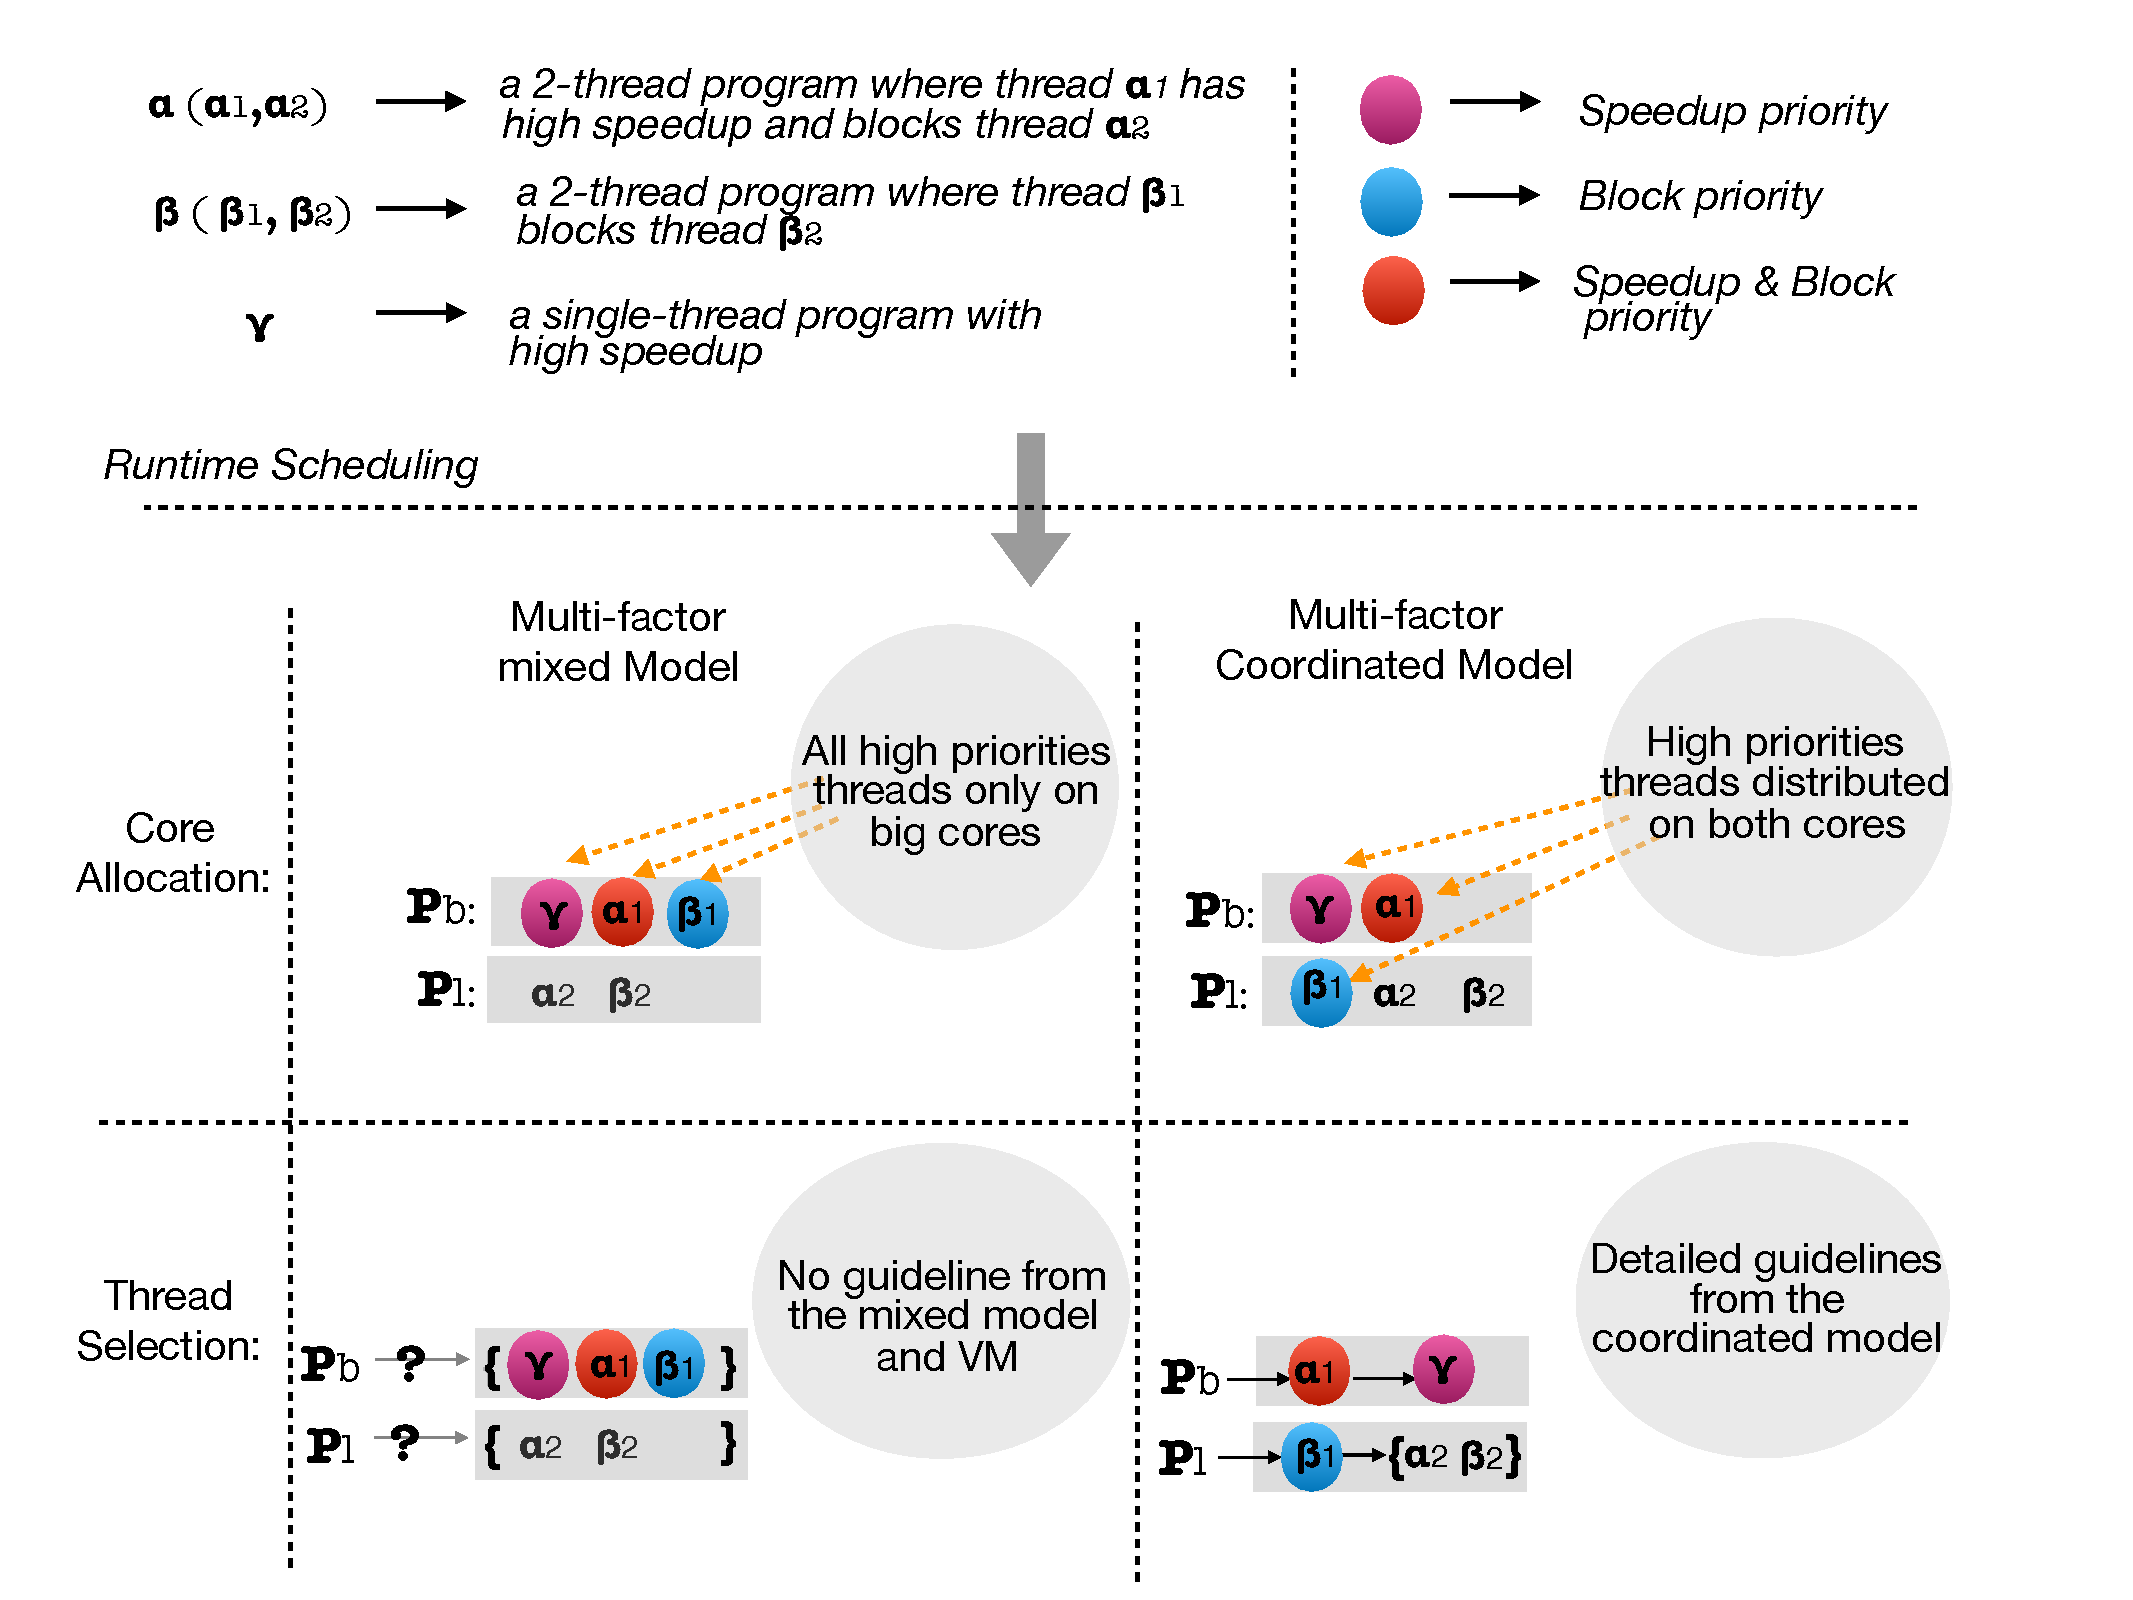
\includegraphics[scale = 0.26]{figures/me.pdf}
\caption{Motivating Example: Multi-threaded multiprogrammed workload on asymmetric multicore processors with one big core $P_b$ and one little core $P_l$. Controlling only core affinity results in suboptimal scheduling decisions.}
\label{me}
\end{figure} 

%In brief, fairness-oriented approaches have demonstrated their efficiency on multiprogram co-executed workloads with single-thread applications as precise mathematical analysis can be constructed \cite{kim2016fairness, kim2018exploring}. Bottleneck acceleration methods equipped with a runtime core sensitivity model have shown significant advantage on multi-thread applications in general single-program workloads \cite{joao2012bottleneck,joao2013utility}. In addition, with more emphasis posed on fairness with help of VM one can also obtain a powerful multi-factor mixed model applied by the state-of-the-art AMP-aware scheduler \cite{jibaja2016portable}. 

%To the best of knowledge, there are two problems remain in the VM-based multi-factor mixed model when it is targeting multi-thread multiprogram scheduling.   
%In brief, single-factor based approach can efficient deal with certain scenarios with limited workloads and runtime but losing generality. Multi-factor based approaches have been shown to be the trend to address general scheduling problem on AMPs with multi-thread workloads. 
%To the best of knowledge, there are two remain problems in the state-of-the-art multi-factor based approach:

\textbf{\textit{Motivating Example:}} To demonstrate the problem, consider the motivating example shown in Figure~\ref{me}. This AMP system has a high performance big core, $P_b$, and a low performance little core, $P_l$. Three applications, {$\alpha$, $\beta$, $\gamma$}, are being executed. $\alpha$ and $\beta$ have two threads.
The first thread of each application, $\alpha_1$ and $\beta_1$, blocks the second thread of their application, $\alpha_2$ and $\beta_2$ respectively. $\gamma$ is a single-threaded application. $\alpha_1$ and $\gamma$ enjoy a high speedup when executed on the big core, $P_b$. WASH~\cite{jibaja2016portable}, the existing state-of-the-art multi-factor heuristic, would likely assign the high speedup thread and the two blocking threads to the big core. The thread selector of $P_b$ has no information about the criticality of the threads assigned to it, so the order of execution depends on the underlying Linux scheduler.

A much better solution is possible if we control both core allocation and thread selection in a coordinated, AMP-aware way. In this case, we map the two threads that benefit the most from the big core, $\gamma$ and $\alpha_1$, to $P_b$, while we map the other bottleneck thread, $\beta_1$, to $P_l$. This will not impact the overall performance of $\beta$. The thread selector knows $\beta_1$ is a bottleneck thread and executes is immediately. So, what we lose in execution speed for $\beta_1$, we gain in not having to wait for CPU time. Similarly, this coordinated policy guarantees that $\alpha_1$ will be given priority over $\gamma$. 

%Based on the multi-factor mixed model \cite{jibaja2016portable}, either the high speedup thread ($\gamma$) or blocking threads ($\alpha_1,\beta_1$) will have affinity on $P_b$ -{\it local-optimal decision}. When the thread selector on $P_b$ is invoked, no more guideline can be obtained from the thread affinity provided by the mixed model - {\it loss of information with mixed priority}. Instead, a better solution can be provided in a multi-factor decentralized model by only mapping the two high speedup threads ($\gamma,\alpha_1$) to $P_b$ and keeping the other blocking thread $\beta_1$ in $P_l$ - {\it global-aware decision}. Then the thread selector invoked by both $P_b$ and $P_l$ guided through the blocking priority, will select and accelerate bottleneck threads $\alpha_1,\beta_1$ locally and simultaneously without waiting each other - {\it sufficient information with precise priority}.  

%both of them will get high priority and be affiliated on the big core. Thus, some of those high priority threads need to be waited in the runqueue of $p_b$. Further, when $p_b$ is ready to select the next task, it may select a $t_s$ first instead of a $t_b$ as the original bottleneck priority has lost after setup its affinity. In brief, the core allocator made the first {\it selfish} greedy decision to enqueue those high priority threads on big core without leaving a better solution space for thread selector. Second, the thread selector lose original information and cannot guarantee to make a good decision. With efficient preemption mechanism, $p_l$ can select a $t_b$ even from $p_b$'s runqueue, but this leads to additional overhead from migration. If the core allocator and thread selector can be collaborated, a trivial better solution in this example can be $p_b$ running \{$t_s \cap t_b$\} whilst $p_l$ running \{$t_b$\}. 

%The first problem is obvious as in runtime scheduling, every change in a current decision will influence the future solution space and there is no way to predict it especially for asymmetric multicore processors with multiple multi-thread workloads.  
%To demonstrate the second problem, scheduling a ready thread from a run-queue in big core to be executed in a ready little core can result in an optimal solution from a greedy point of view, or we say a {\it current} optimal solution. But if this thread will only run on the little core for a tidy bit of time and then move back to a big core by preemption when the big core is ready, the overall runtime overhead from additional migrations may totally defeat the benefit from the hard and useless work on the little core. A high level motivating example is shown in Fig \ref{mt}, where $\mathcal{T}$ is a high priority thread which just ranked in the second position under the current running thread on big core's run-queue. By global scheduling, a ready little core will decide to run this high priority thread $\mathcal{T}$ and migrate it from big core's run-queue. While the problem happens if the big core finish its current thread right after the migration issued by the little core, as the big core will decide to run $\mathcal{T}$ and move it back by preemption. Those frequent runtime selections and migrations do lower the performance in this case.

In this paper, we introduce COLAB, an OS scheduling policy for asymmetric multicore processors that can make such coordinated decisions. Our scheduler uses three collaborating heuristics to drive decisions about core allocation, thread selection, and thread preemption. Each heuristic optimizes primarily one of the factors affecting scheduling quality: core sensitivity, thread criticality, and fairness respectively. Working together, these multi-factor heuristics result in much better scheduling decisions.

We integrated COLAB inside the Linux scheduler module, replacing the default CFS policy for all application threads. We evaluated our policy on multiple big.LITTLE-like simulated systems running 36 distinct workloads, each workload being a random selection of PARSEC3.0, SPLASH2, and SPEC CPU2006 benchmarks. In almost all cases, COLAB was able to improve both turnaround time and throughput compared to the state-of-the-art and the Linux default. In the best case, turnaround time was 50\% less under our policy than under WASH and CFS.

%In brief, our proposed framework equipped with a multi-factor {\it decentralized} model - different runtime factors are distributed to be mainly addressed by different functional units of the scheduler, including core allocator, thread selector and preemption trigger. Decisions in each functional unit are directly guided by priorities from sufficient runtime without losing information through a mixed central model. Those decisions only aim to benefit each of their targeting factors and avoid making trouble for each other, so neither greedy nor local-optimal from a multi-factor point of view. Then all those sub-decisions from different functional units in scheduler dynamically collaborate together to result in overall smarter scheduling decisions during runtime. 

The main contributions of our work are:
\begin{itemize}
\item The first AMP-aware OS scheduler targeting general multi-threaded multiprogrammed workloads.
\item A set of collaborative heuristics for prioritizing thread based on core sensitivity, thread criticality, \emph{and} fairness.
\item Up to 50\% lower turnaround time, 5\% to 28\% on average, compared to the Linux CFS scheduler and WASH.
\end{itemize}

The remainder of this paper is presented as follows: Section 2 describes the background and related work. Section 3 presents our multi-factor collaborative model. We describe its implementation and analyze its operation in Section 4. We evaluate the scheduling police in Section 5, and we summarize and conclude the paper in Section 6.  